\documentclass[border=10pt]{standalone}

\usepackage{tikz}
\usepackage{tikzsymbols}
\usetikzlibrary{calc,patterns,shapes.geometric}

\def\centerarc[#1](#2)(#3:#4:#5){\draw[#1] ($(#2)+({#5*cos(#3)},{#5*sin(#3)})$) arc (#3:#4:#5);}

\begin{document}
	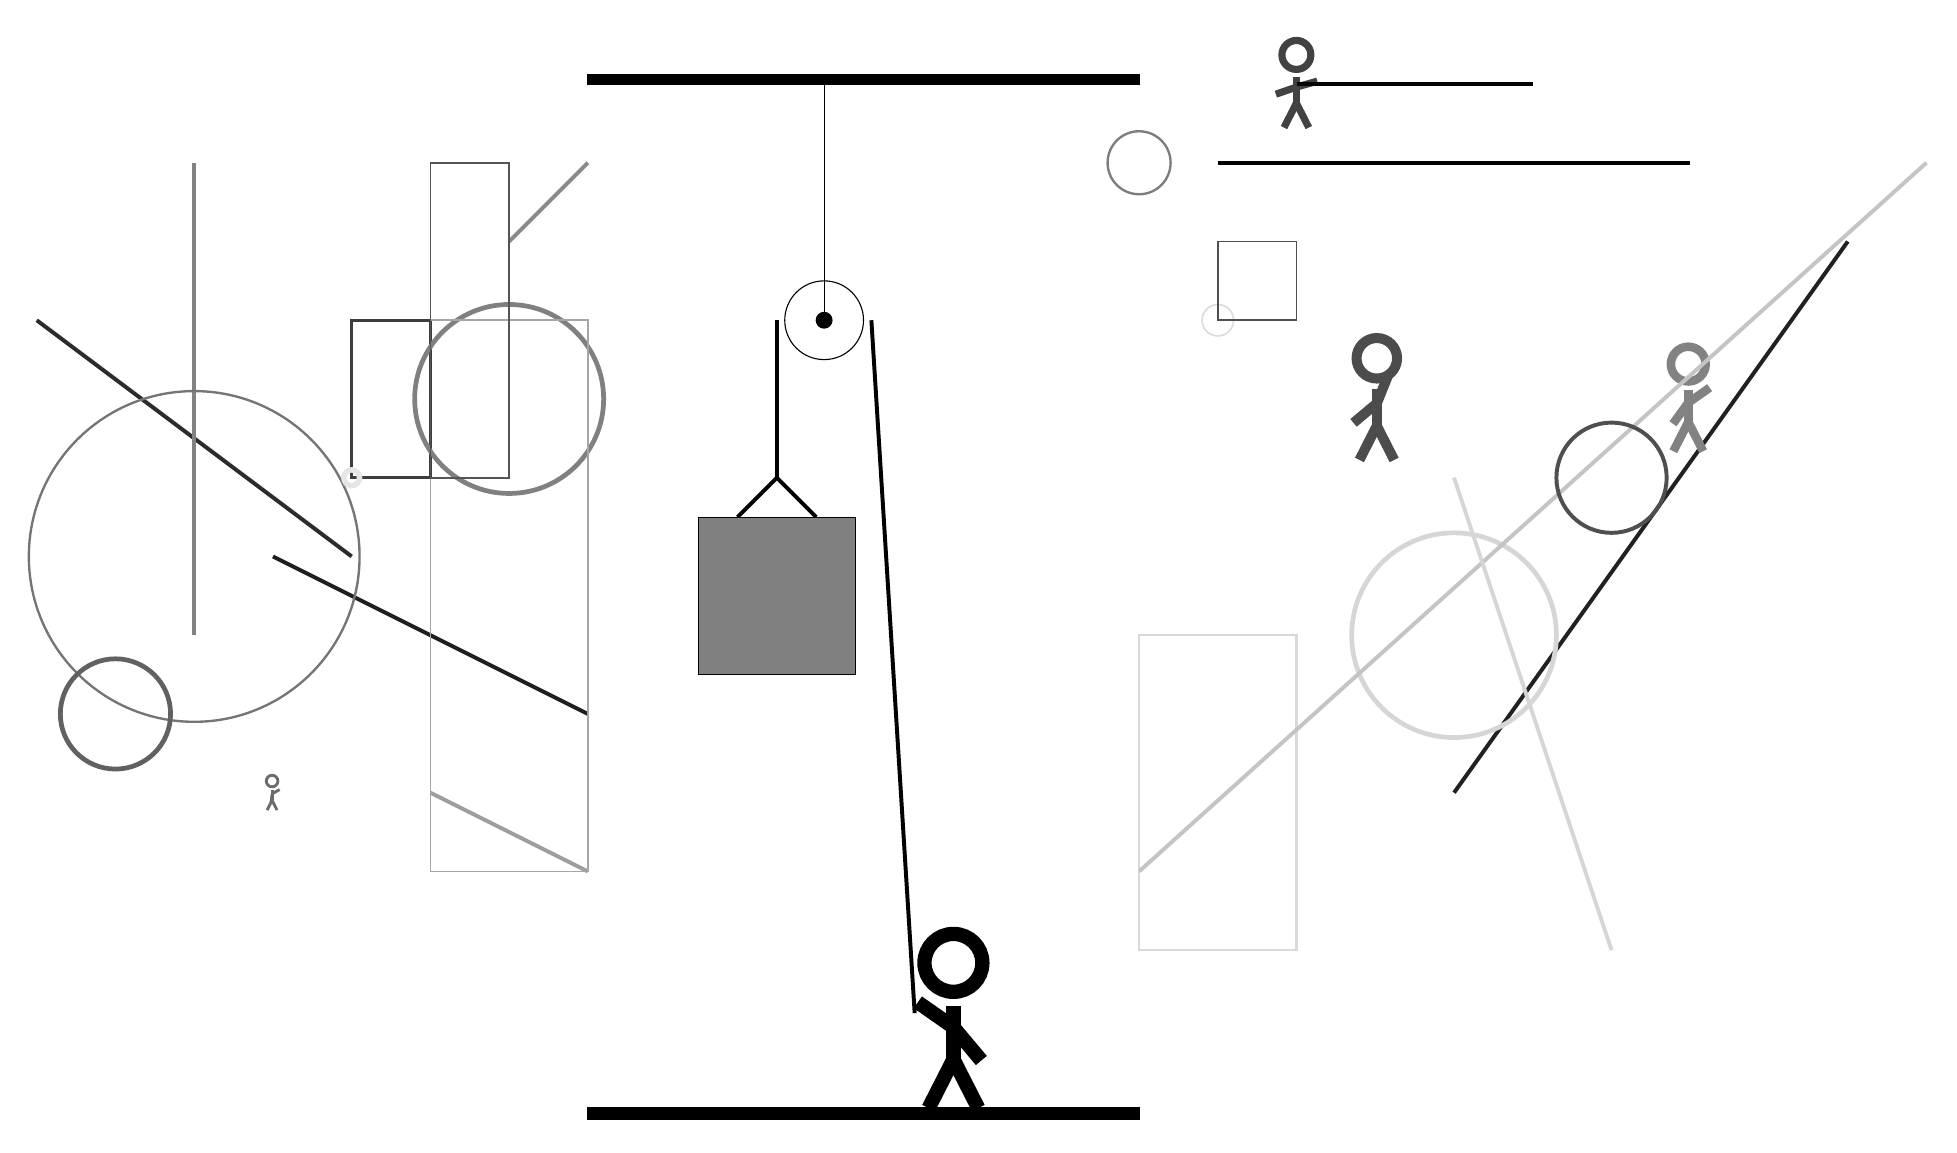
\begin{tikzpicture}
		%%%%% START %%%%%
		
		\draw[fill=black] (-2, 10) rectangle (5, 10.125);
		
		\draw (1, 7) circle (0.5);
		\draw[fill=black] (1, 7) circle (0.1);
		\draw (1, 10) -- (1, 7);
		
		\draw[line width=0.5mm] (-0.1, 4.5) -- (0.4, 5.0) -- (0.9, 4.5);
		\draw[fill=black!50] (-0.6, 4.5) rectangle (1.4, 2.5);
		
		\draw[line width=0.5mm] (0.4, 7) -- (0.4, 5.0);
		\centerarc[line width=0.5mm](1, 7)(0:180:0.6);
		\draw[line width=0.5mm](1.6, 7) -- (2.15, -1.8);
		
		\node at (2.6, -1.9) {\Strichmaxerl[10][-35][-50]};
		
		\node[line width=0.3mm, color=black!58] at (-6, 1) {\Strichmaxerl[2][83][30]};
		
		\draw[line width=0.5mm, color=black!88](-6, 4) -- (-2, 2);
		\draw[line width=0.5mm, color=black!87](9, 1) -- (14, 8);
		\draw[line width=0.5mm, color=black!83](-5, 4) -- (-9, 7);
		\draw [line width=0.3mm, color=black!51](5, 9) circle (0.4);
		\node[line width=0.6mm, color=black!74] at (7, 10) {\Strichmaxerl[5][19][16]};
		\node[line width=0.7mm, color=black!70] at (8, 6) {\Strichmaxerl[7][40][68]};
		
		\draw [line width=0.6mm, color=black!16](9, 3) circle (1.3);
		\draw[line width=0.4mm, color=black!76] (-4, 7) rectangle (-5, 5);
		\draw[line width=0.5mm, color=black!49](-7, 3) -- (-7, 9);
		
		\draw[line width=0.5mm, color=black!99](6, 9) -- (12, 9);
		
		\draw[line width=0.5mm, color=black!38](-4, 1) -- (-2, 0);
		\draw[line width=0.3mm, color=black!15] (7, -1) rectangle (5, 3);
		\draw [line width=0.3mm, color=black!54](-7, 4) circle (2.1);
		\draw [line width=0.2mm, color=black!14](6, 7) circle (0.2);
		\draw[line width=0.2mm, color=black!69] (6, 7) rectangle (7, 8);
		
		\node[line width=0.7mm, color=black!49] at (12, 6) {\Strichmaxerl[6][54][35]};
		\draw[line width=0.5mm, color=black!23](5, 0) -- (15, 9);
		\draw[line width=0.5mm, color=black!99](7, 10) -- (10, 10);
		\draw [line width=0.5mm, color=black!69](11, 5) circle (0.7);
		\draw [line width=0.7mm, color=black!10](-5, 5) circle (0.1);
		
		\draw [line width=0.6mm, color=black!50](-3, 6) circle (1.2);
		
		\draw[line width=0.2mm, color=black!35] (-2, 0) rectangle (-4, 7);
		\draw[line width=0.5mm, color=black!16](9, 5) -- (11, -1);
		\draw [line width=0.6mm, color=black!62](-8, 2) circle (0.7);
		\draw[line width=0.5mm, color=black!46](-2, 9) -- (-3, 8);
		\draw[line width=0.2mm, color=black!67] (-4, 5) rectangle (-3, 9);
		
		\draw[fill=black] (-2, -3) rectangle (5, -3.15);
		
		%%%%% END %%%%%
	\end{tikzpicture}
\end{document}